% SCIENCE Visual Guide 2.0.1 + AI_SKILLS_R5; Akulin--Karlov batch v2.
% Graph traces are visibly heavier than axes. All labels use anchored positions.
\documentclass[border=5pt]{standalone}
\usepackage{fontspec,unicode-math}
\setmainfont{Noto Sans}
\setsansfont{Noto Sans}
\setmathfont{STIXTwoMath-Regular.otf}
\usepackage{tikz}
\usetikzlibrary{arrows.meta,calc,patterns,decorations.pathreplacing,intersections}
\definecolor{ScienceInk}{HTML}{000000}
\definecolor{ScienceCurve}{HTML}{000000}
\definecolor{ScienceAux}{HTML}{000000}
\definecolor{ScienceMuted}{HTML}{000000}
\tikzset{
  axis/.style={draw=ScienceInk,line width=0.75pt,-{Latex[length=2.2mm,width=1.35mm]}},
  axisplain/.style={draw=ScienceInk,line width=0.70pt},
  curve/.style={draw=ScienceCurve,line width=2.15pt,line cap=round,line join=round},
  curveb/.style={draw=ScienceAux,line width=1.95pt,dash pattern=on 6pt off 2.4pt,line cap=round,line join=round},
  curvedash/.style={draw=ScienceAux,line width=1.9pt,dash pattern=on 4pt off 3pt},
  optbeam/.style={draw=ScienceCurve,line width=1.75pt,-{Latex[length=2.2mm,width=1.3mm]}},
  optback/.style={draw=ScienceAux,line width=1.65pt,-{Latex[length=2mm,width=1.2mm]}},
  opt/.style={draw=ScienceInk,line width=1.0pt},
  opticplate/.style={draw=ScienceInk,line width=1.02pt,pattern=north east lines,pattern color=ScienceMuted},
  tick/.style={draw=ScienceInk,line width=0.7pt},
  textlabel/.style={text=ScienceInk,font=\fontsize{15}{18}\selectfont},
  smalllabel/.style={text=ScienceInk,font=\fontsize{13.5}{16.2}\selectfont},
}
\begin{document}
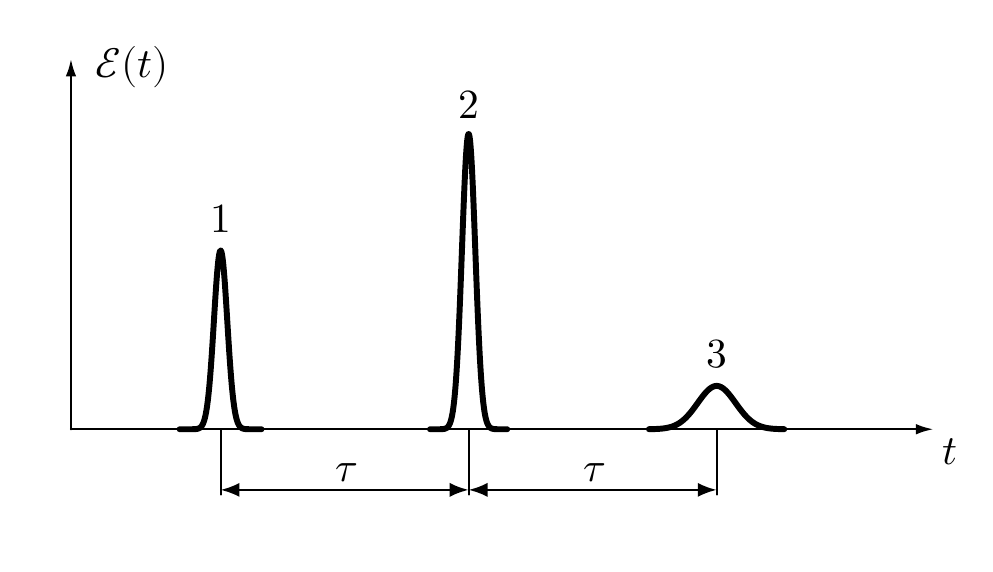
\begin{tikzpicture}[x=1cm,y=1cm,>=Latex,line cap=round,line join=round,font=\fontsize{15}{18}\selectfont]


% Three echoes, τ measured from pulse centrelines; extension lines meet dimension line.
\path[use as bounding box] (0,0) rectangle (11.9,6.55);
\def\Pa{2.45} \def\Delay{3.15}
\pgfmathsetmacro\Pb{\Pa+\Delay}
\pgfmathsetmacro\Pc{\Pb+\Delay}
\draw[axis] (.55,1.45)--(11.5,1.45);
\draw[axis] (.55,1.45)--(.55,6.15);
\node[textlabel,anchor=west] at (.74,6.05) {$\mathscr E(t)$};
\node[textlabel,anchor=west] at (11.5,1.17) {$t$};
\draw[curve,samples=150,domain=1.93:2.97,smooth] plot (\x,{1.45+2.27*exp(-((\x-\Pa)/.12)^2)});
\draw[curve,samples=150,domain=5.11:6.09,smooth] plot (\x,{1.45+3.75*exp(-((\x-\Pb)/.12)^2)});
\draw[curve,samples=130,domain=7.89:9.61,smooth] plot (\x,{1.45+.55*exp(-((\x-\Pc)/.34)^2)});
\node[textlabel,anchor=south] at (\Pa,3.83) {$1$};
\node[textlabel,anchor=south] at (\Pb,5.27) {$2$};
\node[textlabel,anchor=south] at (\Pc,2.10) {$3$};
% Dimensional witness lines from the pulse origin axis, and raised double-ended arrows.
\foreach \x in {\Pa,\Pb,\Pc}{\draw[axisplain] (\x,1.45)--(\x,.62);}
\draw[<->,draw=ScienceInk,line width=.85pt,>=Latex] (\Pa,.68)--node[above,inner sep=2.5pt] {$\tau$}(\Pb,.68);
\draw[<->,draw=ScienceInk,line width=.85pt,>=Latex] (\Pb,.68)--node[above,inner sep=2.5pt] {$\tau$}(\Pc,.68);

\end{tikzpicture}
\end{document}
